\message{ !name(written11.tex)}\documentclass{article}
\usepackage{enumitem}
\usepackage{amsmath}
\usepackage{tikz}
\usepackage[a4paper,
            bindingoffset=0.2in,
            left=0.8cm,
            right=0.8cm,
            top=0.8cm,
            bottom=0.8cm,
            footskip=.25in]{geometry}
\usepackage{fancyhdr}
\begin{document}

\message{ !name(written11.tex) !offset(-3) }

\pagestyle{fancy}
\fancyhf{} % clear existing header/footer entries
\fancyfoot[R]{\fontsize{8}{12}\selectfont \thepage \hspace{0.02cm} of 2}
\fancyfoot[C]{\fontsize{8}{12}\selectfont 1163165}
\fancyfoot[L]{\fontsize{8}{12}\selectfont Javed Alam}


\begin{center}
  \Large\textbf{Mathematics IA - Written 11}\\
  % \large\textit{Javed Alam}
\end{center}
\section*{\fontsize{12}{15}\selectfont Algebra}
\begin{enumerate}[label=(\alph*)]
  \item We will calculate the determinant of the following matrix:
  \begin{center}
  \(A =\) $\begin{bmatrix}
    1 & 2 & 5 & 2 & -1 \\
    2 & 6 & -2 & -4 & -3 \\
    0 & 0 & 1 & 2 & 4 \\
    0 & 0 & 2 & -1 & -3 \\
    0 & 0 & -3 & 1 & 5 \\
  \end{bmatrix}$
\end{center}
This matrix is of the form:
\begin{center}
  \(A =\) $\begin{bmatrix}
  B & D \\
  O & C \\
  \end{bmatrix}$
\end{center}
Where \textit{B} is the square matrix:
\begin{center}
  \(B =\) $\begin{bmatrix}
  1 & 2 \\
  2 & 6 \\
  \end{bmatrix}$
\end{center}
\textit{C} is the square matrix:
\begin{center}
  \(C =\) $\begin{bmatrix}
  1 & 2 & 4 \\
  2 & -1 & -3 \\
  -3 & 1 & 5 \\
  \end{bmatrix}$
\end{center}
and \textit{D} is the matrix:
\begin{center}
  \(D =\) $\begin{bmatrix}
  5 & 2 & -1 \\
  -2 & -4 & -3 \\  
  \end{bmatrix}$
\end{center}
\vspace{.3cm}
As such, the matrix \textit{A} is in block upper triangular form, and thus det\hspace{.04cm}\textit{A} = (det\hspace{.04cm}\textit{B})(det\hspace{.04cm}\textit{C}).
\begin{center}
  \(\lvert B \rvert =\) $\begin{vmatrix}
  1 & 2 \\
  2 & 6 \\
  \end{vmatrix} = 6 - 4 = 2 $
\end{center}
  To calculate det\hspace{.04cm}\textit{C}, we will expand along the first row:
\begin{center}
   \(|C| =\) $\begin{vmatrix}
  1 & 2 & 4 \\
  2 & -1 & -3 \\
  -3 & 1 & 5 \\
  \end{vmatrix}$
  \( =  1\) $\begin{vmatrix}-1 & -3 \\
     1 & 5 
    \end{vmatrix}$ \(- 2\) $\begin{vmatrix}2 & -3 \\ -3 & 5 \end{vmatrix}$ \(+ 4\) $\begin{vmatrix}2 & -1 \\ -3 & 1 \end{vmatrix}$ \\ \vspace{.3cm}
  \(= 1(-2) - 2(1) + 4(-1) = -2 - 2 - 4 = -8\) \\ \vspace{.3cm}  

\end{center}

As such, det\hspace{0.04cm}\textit{A} \(= (2)(-8) = -16\)
\vspace{0.6cm} 
\item Given that \(\vert{G}\vert =\)
$\begin{vmatrix}
  a & b & c \\
  d & e & f \\
  g & h & i \\

\end{vmatrix} = 7$, \textnormal{we will calculate:}
\begin{center}
  \(|H| = \) 
 $\begin{vmatrix} a & b & c \\
  2d & 2e & 2f \\
  g+3a & h + 3b & i + 3c \\
\end{vmatrix}$ 
\end{center} 
\vspace{.3cm}
We can see that the matrix H is row equivalent to G, as it represents the state of G after multiple elementary row operations. Therefore, the determinant can be determined by analysing which row operations were performed. \vspace{0.1cm}

Firstly, the second row has undergone scalar multiplication by 2. This will cause the determinant to be multiplied by 2. Secondly, the third row has had the first row added to it three times. This will not affect the determinant. \\
\vspace{0.1cm} \\
As such, \(\lvert H \rvert = 2\lvert G \rvert = 2(7) = 14\)
\end{enumerate}
\pagebreak
\section*{\fontsize{12}{15}\selectfont Calculus}
We will calculate the following indefinite integral using partial fraction decomposition:
\begin{center}
 \( \displaystyle\int \frac{4x^2 + 2x + 3}{x^3 + x} \hspace{0.1cm} dx\)
\end{center}
We first factorise the denominator:
\begin{center}
\( \displaystyle x^3 + x = x(x^2 + 1)\)
\end{center}
Because $x^2 + 1$ is an irreducible quadratic factor, the partial fraction decomposition will have the form:
\begin{center}
  \( \displaystyle \frac{4x^2 + 2x + 3}{x(x^2 + 1)} = \frac{A}{x} + \frac{Bx + C}{x^2 + 1}\) 
\end{center}
\vspace{0.3cm}
We multiply both sides of the equation by \(x(x^2+1)\) and then calculate the values of $A, B,$ and $C:$
\begin{center}

\( \displaystyle 4x^2 + 2x + 3 = A(x^2+1) + (Bx + C)x \)
\end{center}
\vspace{0.1cm}
Equating coefficients, we can see that $2x = Cx$, and therefore $C = 2$. \hspace{0.01cm}
\vspace{0.2cm} \\*
\hspace{0.01cm}
\vspace{0.2cm}
Additionally, the only constant term on the RHS is A, and so $A = 3$.\\*
\hspace{0.01cm} \vspace{0.03cm}
Finally, as per the squared terms, $4x^2 = Ax^2 +  Bx^2$, and so $B = 4 - 3 = 1$. \vspace{0.5cm} \\*
\hspace{0.01cm} \vspace{0.2cm}
As such, the integral can be expressed as the following sum of two fractions:
\begin{center}
  \( \displaystyle\int \frac{4x^2 + 2x + 3}{x^3 + x} \hspace{0.1cm} dx = \int \frac{3}{x} \hspace{0.1cm} dx + \int \frac{x + 2}{x^2+1} \hspace{0.1cm} dx\)
 \end{center}
 
 \begin{center}
  \( \displaystyle = 3\ln|x| + \int \frac{x+2}{x^2 + 1} \hspace{0.1cm} dx + c\)
 \end{center}
\vspace{0.3cm}
Let $x = \tan(t)$ for $t \in (-\frac{\pi}{2}, 0) \cup (0, \frac{\pi}{2})$ and $x + 2 = \tan(t) + 2,$ then $dx = \sec^2(t)\hspace{0.04cm}dt:$
\vspace{0.3cm}
\begin{center}
  \( \displaystyle 3\ln|x| + \int \frac{x+2}{x^2 + 1} \hspace{0.1cm} dx + c = 3\ln|x| + \int \frac{(\tan(t) + 2)\sec^2(t)}{\tan^2(t) + 1}\hspace{0.1cm}dt + c = 3\ln|x| + \frac{(\tan(t) + 2)\sec^2(t)}{\sec^2(t)}\hspace{0.1cm}dt + c\)
 \end{center}
 \begin{center}
  \( \displaystyle = 3\ln|x| + \int\tan(t) \hspace{0.1cm}dt + 2\int dt + c\) 
 \end{center}
 \begin{center}
  \( \displaystyle = 3\ln|x| + \int\frac{\sin(t)}{\cos(t)}\hspace{0.1cm}dt + 2t + c\) 
 \end{center}
 Let $u = \cos(t),$ then $\frac{du}{dt} = -\sin(t)$ and $dt = -\frac{1}{\sin(t)}\hspace{0.1cm} du:$
 \begin{center}
  \( \displaystyle = 3\ln|x| - \int\frac{1}{u} \hspace{0.1cm}du + 2t + c\) 
 \end{center}

 \begin{center}
  \( \displaystyle = 3\ln|x| - \ln|u| + 2t + c\) 
 \end{center}

 \begin{center}
  \( \displaystyle = 3\ln|x| - \ln|\cos(t)| + 2t + c\) 
 \end{center}
If $\tan(t) = x$ and $t = \arctan(x):$
\begin{center}
  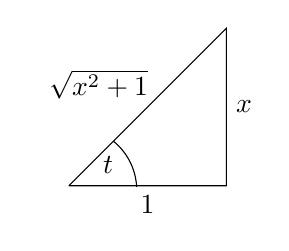
\begin{tikzpicture}
    \draw (0,0)       
      -- (2,0) node[midway, below]{$1$}
      -- (2,1) node[anchor=west]{$x$}
      -- (2,2) 
      -- (1,1) 
      -- (0,0) -- ++(45:0.8cm) arc (-129:-177.1:-0.8cm)
         (9/7,9/7)node[anchor=east, inner sep=1.8ex]{$\sqrt{x^2 + 1}$}  
         (1/2,1/2) node[anchor=north]{$t$};
    \end{tikzpicture}
\end{center}
With reference to the right triangle, $\cos(t) = \frac{1}{\sqrt{x^2+1}}$, and therefore:
\begin{center}
  \( \displaystyle 3\ln|x| - \ln|\cos(t)| + 2t + c = 3\ln|x| - \ln|\frac{1}{\sqrt{x^2+1}}| + 2\arctan(x) + c\) 
 \end{center}
 \begin{center}
  \( \displaystyle = 3\ln|x| - \ln|1| + \ln|\sqrt{x^2+1}| + 2\arctan(x) + c\) 
 \end{center}
 \begin{center}
  \( \displaystyle = \ln|x^3\sqrt{x^2+1}| + 2\arctan(x) + c\) 
 \end{center}
 \begin{center}
  \( \displaystyle = \frac{1}{2}\ln|x^8+x^6| + 2\arctan(x) + c\) 
 \end{center}
 Because $x^8 + x^6$ is never negative, the absolute value function is not required:
 \begin{center}
  \( \displaystyle \int \frac{4x^2 + 2x + 3}{x^3 + x} \hspace{0.1cm} dx = \frac{1}{2}\ln({x^8+x^6}) + 2\arctan(x) + c\) 
 \end{center}

\end{document}
\message{ !name(written11.tex) !offset(-207) }
